\newpage
\section{Création d'une ligne de signes : \tkzcname{tkzTabLine}}
\subsection{Définition}

\begin{NewMacroBox}{tkzTabLine}{\oarg{local options}\var{s(1),...,s(2n-1)}}
  $n$ est le nombre d'éléments du second argument de \tkzname{tkzTabInit}.

\medskip
\begin{tabular}{lll}
\toprule
symbole de rang impair &  & définition \\
\midrule
\TAline{z} {}  {place un trait en pointillés et un zéro centré}
\TAline{t} {}  {place un trait en pointillés centré}
\TAline{d} {}  {place une double barre centrée}
\TAline{\BS textvisiblespace}{} {aucune action }
\bottomrule
\end{tabular}

\medskip
\begin{tabular}{lll}
\toprule
symbole de rang pair & & définition                   \\
\midrule
\TAline{h}  {}  {zone interdite}
\TAline{+}  {}  {le signe $+$}
\TAline{-}  {}  {le signe $-$}
\TAline{\BS textvisiblespace}{} {aucune action }
\bottomrule

\end{tabular}


\medskip
\noindent\emph{\tkzcname{tkzTabLine} accepte  comme argument une liste constituée de symboles. Dans une utilisation \tkzname{normale}, les symboles font partie de   deux catégories; les symboles de rang impair et les symboles de rang pair. Cette distinction est due au fait que les symboles de rang impair sont en général des traits (filets) et ceux pour les places de rang pair sont en général des signes \og $+$ ou $-$ \fg. Les symboles de rang impair agissent graphiquement, et permettent de tracer des filets verticaux. L'argument de \tkzcname{tkzTabLine} en contient \tkzname{$n$} si on suppose que le deuxième argument de  \tkzcname{tkzTabInit} possède \textcolor{red}{$n$} éléments (antécédents). Les symboles de rang pair  permettent d'obtenir un signe \og $+$ ou $-$ \fg\ ou bien une zone interdite (hachurée ou colorée). Chaque ligne de signes en contient \tkzname{$n-1$} et contiendra donc un total de \tkzname{$2n-1$} éléments, c'est à dire \tkzname{$2n-2$} virgules !\\
Les différents symboles "reconnus" sont donnés dans le tableau ci-dessus,  mais vous devez savoir que l'on peut mettre pratiquement n'importe quoi. Cependant attention! la virgule \textcolor{red}{(,)} est le séparateur de liste aussi vous devez prendre des précautions pour introduire un nombre à virgule. Vous avez plusieurs possibilités~:
\begin{itemize}
\item[--] \{4,5\} on place le nombre entre des accolades.
\item[--] \tkzcname{numprint\{4,5\}} ou encore  \tkzcname{np\{4,5\}}, ce qui nécessite de charger l'excellent package \tkzname{numprint}\NamePack{numprint} avec l'option \tkzname{np} pour le raccourci.
\end{itemize}}

\medskip
\begin{tabular}{lllc}
\toprule
options   & défaut       & définition         \\
\midrule
\TOline{style}  {dotted    } {style des traits verticaux                }
\TOline{help}   {no default} {affiche la structure d'une ligne de signes}
\bottomrule
\end{tabular}

\medskip
\noindent\emph{Il est possible de changer localement le style des filets verticaux et il est possible d'avoir des renseignements sur la structure de la ligne.}
\end{NewMacroBox}

\subsection{Nombre d'arguments utilisés.}
La syntaxe générale est :

\begin{tkzltxexample}[]
 \tkzTabInit{ e(1),...,e(i),...,e(p)} % tableau à p lignes.
            { a(1),...,a(i),...,a(n)} % n antécédents
 \tkzTabLine{ s(1),...,s(i),...,s(2n-1)}
\end{tkzltxexample}


\medskip
Si on utilise \tkzname{$n$} antécédents pour la première ligne alors il y aura \tkzname{$n$} symboles de rang impair et \tkzname{$n-1$} symboles de rang pair, soit \tkzname{$2n-1$} symboles.

 Les principaux symboles  utilisés sont : \tkzname{z} pour un zéro placé sur un trait, \tkzname{t} pour un trait correspondant  à un zéro d'une autre ligne, \tkzname{d} pour une valeur pour laquelle l'expression n'est pas définie.

Voyons une illustration  simple : trois antécédents $a_1$, $a_2$, et $a_3$ permettront de mettre $2\times3 -1 =5$ symboles. Les $3$ valeurs de la première ligne impliquent pour l'argument de   \tkzcname{tkzTabLine} de posséder {$2\times 3-1=5$} éléments  c'est-à-dire être une liste comportant   $3$ symboles de rang impair et $2$ symboles de rang pair, soit un total de $5$ symboles qui seront séparés par $4$ virgules.

\begin{center}
  \begin{tikzpicture}
    \tkzTabInit[espcl=3,lgt=2]%
    {\colorbox{red!40}{\textcolor{white}{$x$}}    / 1,%
     \colorbox{red!40}{\textcolor{white}{$f(x)$}} / 1}%
    {\colorbox{blue!40}{\textcolor{white}{ $a_1$}},%
     \colorbox{blue!40}{\textcolor{white}{ $a_2$}},%
     \colorbox{blue!40}{\textcolor{white}{ $a_3$}}}%
    \path (N11)--(N12) node[circle,draw, fill= lightgray,midway] {1};
    \path (N12)--(N21) node[midway] {$,$};
    \path (N21)--(N22) node[circle, draw, fill= lightgray,midway] {3};
    \path (N31)--(N32) node[circle,draw,  fill= lightgray,midway] {5};
    \path (M11)--(M12) node[circle, draw, fill= orange!30,midway] {2};
    \path (M21)--(M22) node[circle,draw,  fill= orange!30,midway] {4};
  \end{tikzpicture}
\end{center}

Pour obtenir cette ligne, il faut entrer
\begin{tkzexample}[code only]\tkzTabLine{ $1$ , $2$ , $3$ , $4$ , $5$}
\end{tkzexample}





\subsection{Emploi minimum}
La deuxième ligne est vide mais l'argument \tkzcname{tkzTabLine} doit comporter \tkzname{$4$} virgules. C'est en effet une liste comportant \tkzname{$5 = 2\times3-1$} valeurs.

\begin{tkzexample}[code only]
 \tkzTabLine{,,,,} ou \tkzTabLine{ , , , , }\end{tkzexample}

\begin{tkzexample}[width=8cm,small]
\begin{tikzpicture}
  \tkzTabInit[espcl=1.5]
     {$x$  / 1 ,$f(x)$ /1 }%
     {$v_1$ , $v_2$ , $v_3$ }%
  \tkzTabLine{ , , , , }
\end{tikzpicture}
\end{tkzexample}

\subsubsection{\texttt{\textcolor{red}{t}} : ajout d'un trait}
Cette option place un simple trait verticalement.
\begin{tkzexample}[width=8cm,small]
\begin{tikzpicture}
  \tkzTabInit[espcl=1.5]
     {$x$  / 1 ,$f(x)$ /1 }%
     {$v_1$ , $v_2$ , $v_3$ }%
  \tkzTabLine{ t, , t , ,t }
\end{tikzpicture}
\end{tkzexample}

\subsubsection{\texttt{\textcolor{red}{z}} : ajout d'un zéro sur un trait vertical}
\begin{tkzexample}[width=8cm,small]
\begin{tikzpicture}
  \tkzTabInit[espcl=1.5]
     {$x$  / 1 ,$f(x)$ /1 }%
     {$v_1$ , $v_2$ , $v_3$ }%
  \tkzTabLine{ z, , z , ,z }
\end{tikzpicture}
\end{tkzexample}

\subsubsection{\texttt{\textcolor{red}{d}} : double barre}

On peut aussi avoir le cas d'une fonction  non définie en $0$ et en $2$ mais s'annulant en $1$. On place à chaque extrémité le symbole |d|.

\begin{tkzexample}[width=7cm,small]
\begin{tikzpicture}
  \tkzTabInit[espcl=1.5]%
    {$x$ / 1,$g(x)$ / 1}%
    {$0$,$1$,$2$}%
\tkzTabLine{d,+,0,-,d}
\end{tikzpicture}
\end{tkzexample}

On peut aussi avoir le cas d'une fonction admettant une dérivée à droite différente de la dérivée à gauche

\begin{tkzexample}[width=7cm,small]
\begin{tikzpicture}
   \tkzTabInit[lgt=1.5,espcl=1.75]%
       {$x$ / 1,$f'(x)$ / 1}%
       {$-\infty$,$0$,$+\infty$}%
   \tkzTabLine{,+,d,-,}
\end{tikzpicture}
\end{tkzexample}

\subsection{Utilisation des symboles de rang pair}

Pour un tableau de signe, en principe les symboles de rang pair mais il est possible de détourner l'emploi de base de cette macro. L'exemple suivant montre un cas classique d'une zone du tableau qui correspond à des valeurs interdites. par défaut avec le symbole \tkzname{h}, la zone est grisée mais on peut hachurer cette zone si on préfère.
Le dernier exemple montre comment détourner l'usage principal.

\subsubsection{\texttt{\textcolor{red}{h}} : zone interdite}

Une fonction peut ne pas être définie sur un intervalle, ici $[1~;~2]$. La partie du tableau qui correspond à cet intervalle sera hachurée ou bien colorée (par défaut, la zone est grisée). Des options permettant de personnaliser seront offertes. Pour l'exemple suivant, il suffit de placer |h| entre les deux |d| qui correspondent aux valeurs interdites\index{valeurs interdites} $1$ et  $2$.

\begin{tkzexample}[width=8cm, small]
\begin{tikzpicture}
  \tkzTabInit[color,espcl=1.5]
  {$x$ / 1,$g(x)$ / 1}
  {$0$,$1$,$2$,$3$}%
  \tkzTabLine{z, + , d , h , d , - , t}
\end{tikzpicture}
\end{tkzexample}

\subsection{Utilisation des options}

\subsubsection{\tkzname{t style} : modification du style des traits verticaux}
\Istyle{tkzTabLine}{t style}

\begin{tkzexample}[width=7cm, small]
\begin{tikzpicture}
\tikzset{t style/.style = {style = dashed}}
  \tkzTabInit[espcl=1.5]
     {$x$  / 1 ,$f(x)$ /1 }%
     {$v_1$ , $v_2$ , $v_3$ }%
  \tkzTabLine{ t, , t , ,t }
\end{tikzpicture}
\end{tkzexample}


\begin{tkzexample}[width=7cm, small]
\tikzset{t style/.style = {style = densely dashed}}
\begin{tikzpicture}
  \tkzTabInit[espcl=1.5]
     {$x$  / 1 ,$f(x)$ /1 }%
     {$v_1$ , $v_2$ , $v_3$ }%
  \tkzTabLine{ z, , z , ,z }
\end{tikzpicture}
\end{tkzexample}

\subsubsection{\tkzname{help} : Affiche la structure du tableau}
\Iopt{tkzTabLine}{help}
Voir la section \og personnalisation \fg\ (\ref{pers}).


\subsection{Utilisation des styles}

\subsubsection{\tkzname{h style} : modification de la couleur d'une zone interdite}
\Istyle{tkzTabLine}{h style} \index{zone interdite}
Si vous préférez hachurer une zone du tableau, alors  il faut modifier un style.
\begin{tkzexample}[width=8cm,small]
\begin{tikzpicture}
  \tikzset{h style/.style = {fill=red!50}}
  \tkzTabInit[color,espcl=1.5]%
    {$x$ / 1,$g(x)$ / 1}%
    {$0$,$1$,$2$,$3$}%
  \tkzTabLine{z,+,d,h,d,-,t}
\end{tikzpicture}
\end{tkzexample}


Cette fois la zone est hachurée.
 \index{hachures}
\begin{tkzexample}[width=8cm,small]
\begin{tikzpicture}
  \tikzset{h style/.style =
          {pattern=north west lines}}
  \tkzTabInit[color,espcl=1.5]%
    {$x$ / 1,$g(x)$ / 1}%
    {$0$,$1$,$2$,$3$}%
  \tkzTabLine{z,+,,h,d,-,t}
\end{tikzpicture}
\end{tkzexample}



\subsection{Exemples}

\subsubsection{Simplification d'une expression comportant une valeur absolue }

\begin{tkzexample}[width=8cm,small]
 \begin{tikzpicture}
 \tkzTabInit[lgt=2,espcl=1.75]%
  {$x$/1,$2-x$/1, $\vert 2-x \vert $/1}%
  {$-\infty$,$2$,$+\infty$}%
 \tkzTabLine{ , + , z , - , }
 \tkzTabLine{ , 2-x ,z, x-2, }
\end{tikzpicture}
\end{tkzexample}

\subsubsection{Tableau de signes}

\begin{tkzexample}[ small]
\begin{tikzpicture}
  \tkzTabInit[lgt=3,espcl=1.5]%
     {$x$                                   /1,
      $x^2-3x+2$                            /1,
      $(x-\E)\ln x$                   /1,
      $\dfrac{x^2-3x+2}{(x-\E)\ln x}$ /2}
              {$0$  , $1$  , $2$  , $\E$  ,$+\infty$}
              \tkzTabLine{ t,+,z,-,z,+,t,+,}
              \tkzTabLine{ d,+,z,-,t,-,z,+,}
              \tkzTabLine{ d,+,d,+,z,-,d,+,}
\end{tikzpicture}
\end{tkzexample}


\subsubsection{Signe d'une expression du second degré}

Si $\Delta  \geq 0$ on peut écrire  $\displaystyle ax^2+bx+c=a\left(x-\dfrac{-b-\sqrt{b^2-4ac}}{2a}\right)\left(x-\dfrac{-b+\sqrt{b^2-4ac}}{2a}\right)$


\begin{tkzexample}[vbox,small]
\begin{tikzpicture}
 \tkzTabInit[color,lgt=5,espcl=3]%
   {$x$ / .8,$\Delta>0$\\ Le signe de\\ $ax^2+bx+c$ /1.5}%
   {$-\infty$,$x_1$,$x_2$,$+\infty$}%
 \tkzTabLine{ , \genfrac{}{}{0pt}{0}{\text{signe de}}{a}, z
              , \genfrac{}{}{0pt}{0}{\text{signe}}{\text{opposé de}\ a}, z
              , \genfrac{}{}{0pt}{0}{\text{signe de}}{a},  }
 \end{tikzpicture}
\end{tkzexample}
 Il faut noter l'emploi de la macro \tkzcname{genfrac}\footnote{\tkzcname{genfrac} est une macro du package \tkzname{amsmath}}.

\medskip
Si $\Delta  = 0$ alors on peut écrire   $\displaystyle ax^2+bx+c=a\left(x+\dfrac{b}{2a}\right)^2$

\begin{tkzexample}[vbox,width=7cm,small]
\begin{tikzpicture}
  \tkzTabInit[color,lgt=5,espcl=3]%
   {$x$ / 1 , $\Delta=0$\\ Le signe de\\ $ax^2+bx+c$  / 2}%
   {$-\infty$,$\dfrac{-b}{2a}$,$+\infty$}%
  \tkzTabLine{ , \genfrac{}{}{0pt}{0}{\text{signe de}}{ a} , z
               , \genfrac{}{}{0pt}{0}{\text{signe de}}{a}, }
\end{tikzpicture}
\end{tkzexample}

Si $\Delta  < 0$  alors  $\displaystyle ax^2+bx+c=a\left[\left(x+\dfrac{b}{2a}\right)^2 -\dfrac{b^2-4ac}{4a^2}\right]$

\begin{tkzexample}[vbox,width=7cm,small]
\begin{tikzpicture}
  \tkzTabInit[color,lgt=5,espcl=5]%
   {$x$/.8,$\Delta<0$\\ Le signe de\\ $ax^2+bx+c$/2}%
   {$-\infty$,$+\infty$}%
 \tkzTabLine{ , \genfrac{}{}{0pt}{0}{\text{signe de}}{ a}, }
\end{tikzpicture}
\end{tkzexample}


\endinput